\section{The \specula protocol}
\label{sec:protocol}
This section presents the \specula protocol. First (\S \ref{sub:overview}), we give an overview of the protocol's execution and introduce the key techniques that distinguish it from conventional transactional protocols. Next (\S \ref{subsec:execution}), we delve into the detail of the protocol. Finally, we discuss the fault tolerance of \specula and the algorithm of the automatic tuning method.

\iffalse
\subsection{Transaction execution}
Figure \ref{fig:txn_state} presents the execution state diagram of a speculative transaction.

\begin{figure}[t]
\centering
\hspace{-6mm}
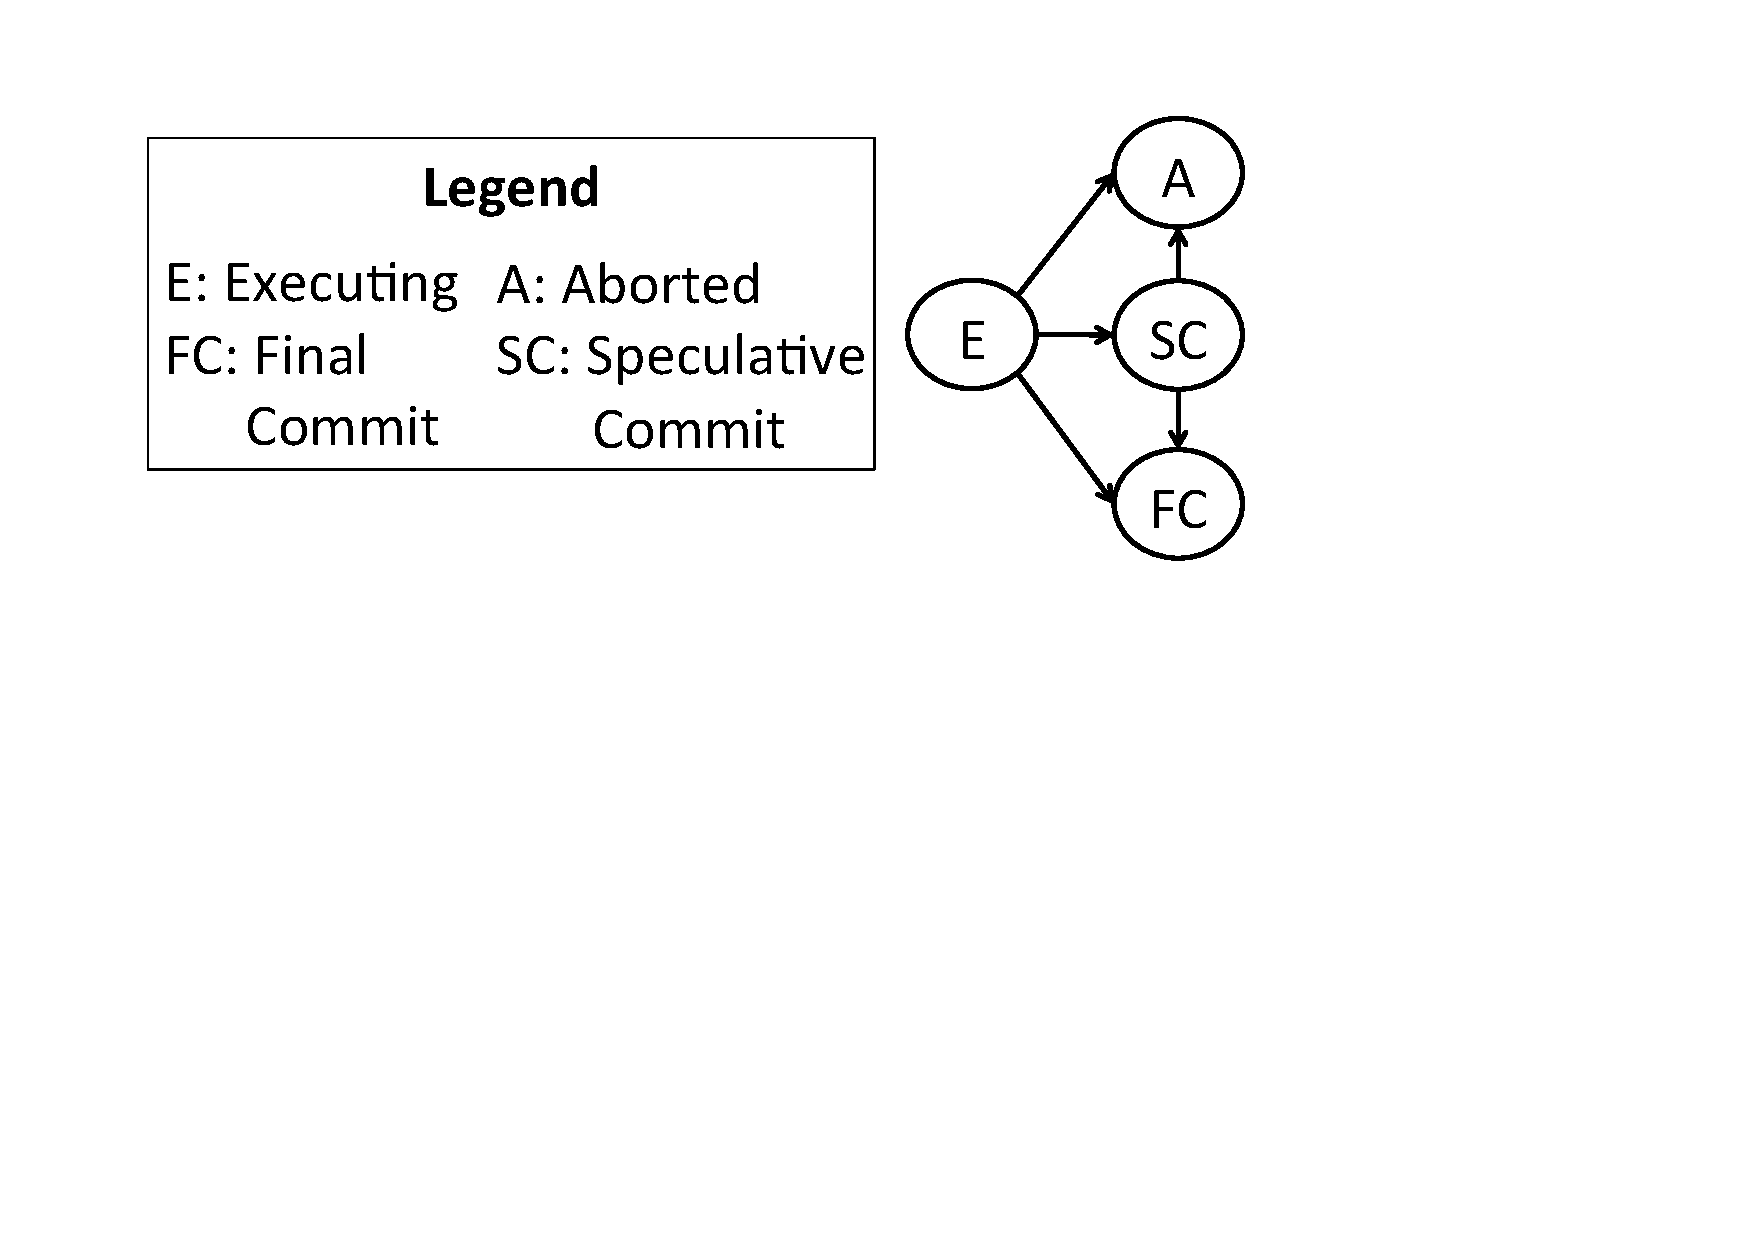
\includegraphics[scale = 0.3]{figures/state-machine.pdf}
\caption{Diagram illustrating the possible state transitions of a transaction in \specula.}
\label{fig:txn_state}
\end{figure}


\begin{figure}[t]
\centering
\begin{subfigure}[t!]{0.95\linewidth}
\def\svgwidth{0.95\columnwidth}
\centering 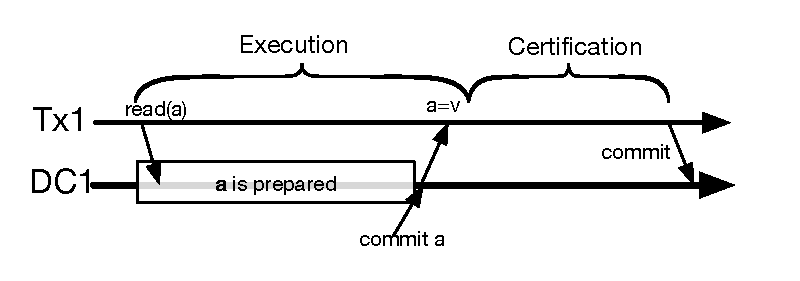
\includegraphics[scale = 0.55]{figures/NoSpeculativeRead}
\vspace{-4mm}
\caption{\footnotesize Not allowing reading pre-commit values.}
\label{fig:remote:a}
\end{subfigure}

\begin{subfigure}[t!]{0.95\linewidth}
\vspace{1mm}
\def\svgwidth{0.95\columnwidth}
\centering 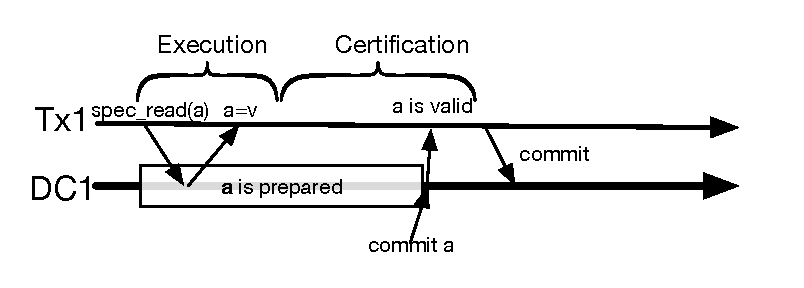
\includegraphics[scale = 0.55]{figures/YesSpeculativeRead}%Remotereadremoteread
\vspace{-4mm}
\caption{\footnotesize Speculatively reading pre-commit values.}
\label{fig:remote:b}
\end{subfigure}
\caption{\small The execution path of enabling or disabling speculative read.}
\label{fig:specularead}
\end{figure}
\fi


\subsection{Protocol overview}
\label{sub:overview}
At its core, {\specula} is based on a transactional protocol that provides Snapshot Isolation \cite{clocksi, ports2012serializable}, executed on top of a (partially) replicated datastore. Here, we briefly depict the execution of the baseline protocol: firstly, a transaction is initialized in a datacenter, then the transaction issues a sequence of read and write operations; after the execution phase, the transaction's coordinator sends its write-set to its master partitions for certification; after certifying the write-set, a master partition replicates the prepared records to its replicas synchronously, and replicas directly acknowledge the transaction coordinator; finally, the coordinator commits the transaction after it received replies from all replicas of involved partitions. This baseline execution constitutes 

Additional to the conventional SI semantics (which is required for transactions that final commit), \specula employs several key techniques to exploit the performance benefit of speculative execution while still providing stringent guarantees, as in the following sub-sections.

\subsubsection{Internal speculative commit}
\label{subsubsec:isc}
As have been described in \S \ref{sec:introduction}, naively allowing transactions to read any pre-commit records can expose non-atomic, non-isolated snapshots to applications, which are perceived as concurrency anomalies and may even hamper application execution. \specula employs a \textit{local certification} phase to guarantee that the produced atomic and isolated speculative states locally. After the execution phase, rather than directly certifying a transaction's write-set at its master partitions, \specula conducts a local certification phase: the updated keys of the transaction are certified at their corresponding local owning partitions (or at a special cache partition if a key is not replicated locally), against committed transactions and speculatively-committed transactions (to ensure SPSI Property 3). If the transaction passes local certification phase, the transaction's updates are atomically applied locally. This process, namely \textit{internal speculative commit}, is conducted for all update transactions, in order to ensure that the speculative states of a node contains atomic updates of a transaction, and no conflicting transactions can co-exist. Unless a programmer allows returning the transaction's speculative commit to clients, this process is totally transparent to clients.

\subsubsection{Minimizing transaction's commit time for speculative read}
\label{subsec:pc}
A transaction can read updates of locally speculative-commit transactions with timestamps smaller than its snapshot time, based on an optimistic guess that the pre-commit data versions will commit with timestamps below the reader's snapshot. Therefore, the reader transaction can proceed execution and enter certification phase, but it can not commit unless knowing that all transactions it has read from commit with timestamps than its snapshot, i.e. \textbf{data dependencies} are resolved. When data dependencies turn to be all valid, speculative read can save large execution, and even certification, latency. On the other hand, aborting due to reading invalid values results in a waste of computation. 

However, despite transaction's abort rate, the underlying commit timestamp assignment scheme also effects for the benefits of speculative read: even if transactions has high commit rate, if they are always assigned large commit timestamps, their readers are still likely to be aborted. Ideally, a timestamp assignment scheme should assign commit timestamps as small as possible, as long as it does not violate SI and SPSI. However, as far as we know, the commit timestamp assignment schemes of existing state-of-the-art decentralized transactional protocols \cite{clocksi, spanner} do not meet this requirement. These protocols store a scalar clock (either physical, logical or hybrid) per data partition, which keeps track timestamps of events that have involved this partition, and proposes monotonically increasing timestamp when preparing a transaction. Then, the commit timestamp of a transaction is calculated as the maximal of proposed prepare time. As each partition has only one scalar clock, all transactions involving this partitions inflate the value of the timestamp, causing large prepare timestamp to be proposed. To mitigate this problem, we propose a time assignment scheme, namely \textit{PreciseClock}, that produces small logical duration for transactions. Essentially, we keep a scalar clock per key and use the scalar clock to track precisely the timestamp of read/write events happened to a key, to propose a timestamp that is only necessarily large to not violate properties of SI and SPSI. Note that the reduction of commit timestamp brought by PreciseClock is especially beneficial for speculative reads, but it can also reduces abort rate for workloads not permitting speculative reads. We present the execution rules of PreciseClock and explain its use in the protocol execution.
\begin{itemize}
\item \textbf{Read} When a transaction $T_x$ reads a key K, it is blocked if K is currently being prepared with a prepare time smaller than $T_x$'s snapshot ($ST_x$). Otherwise, $Tx$ reads K's highest version below $ST_x$ and updates K's high time (HT) to $max(HT, ST_x)$.
\item \textbf{Prepare} When preparing K, a transaction $T_y$ gets prepare time as $max(HT, ST_y)+1$. $T_y's$ commit timestamp is the maximal of the prepare time for all keys of its write-set.
\end{itemize}

\iffalse
\begin{figure}[tbh]
\centering
\hspace{-6mm}
\centering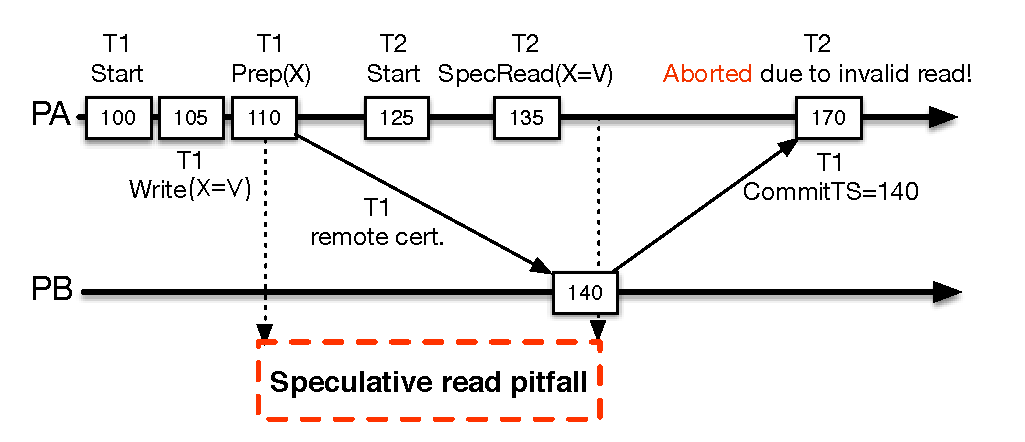
\includegraphics[scale = 0.48]{figures/SpeculativeRead}
\caption{\textit{Transaction reading an invalid prepared version.} Horizontal lines denote two distant partitions PA and PB. Numbers in boxes denote a partition's physical time.}
\label{fig:specula_read}
\end{figure}


\textit{PreciseClock} strikes to propose small prepare timestamps, while not violating any properties of SI or SPSI. On the contrary, we find that the current timestamp assignment scheme proposes unnecessarily large prepare timestamps. Protocols like \cite{clocksi, spanner} enforce each partition to propose monotonically-increasing (physical) timestamps than previous received events (timestamps of read and prepare). In essence, this ensures that after a transaction read a key from a partition, further transactions that update that key can only commit with a larger timestamp than the previous reader's snapshot time, so that the reader's snapshot remains unchanged and thus consistent. However, under this rule, even transactions that update disjoint keys will get higher timestamp than the reader's snapshot time. It is easy to see that this is not necessary: imagine the current protocol is applied to a datastore where each partition only contains a single key; in that case, non-conflicting transactions, which would access the same partition due to data placement, will access disjoint partitions and get different timestamps. Based on this intuition, we propose a new scheme that \textbf{precisely} tracks the read/write causal relations and tries to propose minimal prepare time. We combine the use of physical and logical clocks (as in \ref{hybridclock, bravoclock}): our scheme still uses physical time as a transaction's snapshot time, but maintains a logical clock per key to track the timestamp of transactions that have read the key, i.e. \textit{high time}.
\fi

\iffalse
 and we will discuss its correctness.
\fi

\subsubsection{Pipelining speculative transactions}
\label{subsec:pipeline}
As have been discussed in \S \ref{subsubsec:isc}, each update transaction is firstly locally certified and then applied to the local storage, i.e. it passes internal speculative commit. As can be controlled through the API, if the developer is willing to take risk for reducing latency and increasing throughput, the system can externalize speculative commit of transactions to end-users. The end-users, which can either be human users or some process, can issue new transactions, while the previous one is still being certified. The pipelined speculative transactions issued by a user may have potential causal dependencies: for example, if a user issued two speculative transactions to book a flight and then to book a hotel room, the second transaction should not succeed unless the first succeeds. To capture this relation, \textbf{flow dependence} is created for a client's pipelined speculative transactions: if a speculative transaction is aborted, the client's other transactions issued after the aborted one will be aborted; moreover, a transaction can not commit before its previous speculative transactions commit. The maximal number of speculative transactions a client can pipeline, i.e. \textbf{speculation chain length}, is non-trivial choice that can greatly impact performance: larger speculation length gives clients more opportunity to overlap local computation with synchronization, but also leads to high cost when cascading abort happens; smaller length limits the damage of cascading abort, but also restrict the chance of pipelining more transactions. Instead of placing burdens on developers to reason about this, we propose a simple, yet effective self-tuning algorithm. The detail of the algorithm will be described in \S \ref{subsec:tuning}.

\subsection{Speculative protocol execution}
\label{subsec:execution}
\paragraph{Start transaction and execution} As in the baseline protocol, a transaction is initialized in a server and assigned the server's physical time as its snapshot time (Alg1, lines 1-3). Then it performs a sequences of read and write operations.

\paragraph{Local certification} After the execution all operations, the transaction undergoes the local certification phase. To enforce SPSI property 3, the transaction's updated keys are sent to their local replicated partitions (no matter the partition is a master or slave replica) to check write-write conflict with committed and speculatively committed transactions. Keys not replicated locally are sent to a local cache partition, which temporarily stores speculative updates to non-local keys created by previous local speculative transactions (Alg1, lines 12-13). A partition replies \textbf{abort} in case conflicts are detected; otherwise, the partition prepares the transaction and proposes a prepare timestamp according to the PreciseClock rule: for each key, it retrieves the key's $HighTime$ and proposes $HighTime+1$; then the maximal of proposed time for all keys is returned as the prepare timestamp (Alg2, lines 21-23). Essentially, a transaction passed local certification is ensured that, among all keys replicated locally (and temporarily cached keys), the transaction has no conflict with committed transactions and local speculative transactions. Note that at this point, these prepared records are still not visible to other local transactions, as they may be prepared with different timestamps and allowing them to be visible already could violate consistent snapshot.

\iffalse
the transaction coordinator also certifies all keys belonging to local slave partitions and the cache (which contains all keys of speculatively-committed transactions locally, as will be explained in following text), against locally prepared or speculatively-committed transactions and committed transactions (Alg1, line 13). The local cache only temporarily caches speculative updates for local transactions to read. If a transaction's write-set does not conflict with (i.e. overlaps in duration) existing prepared or speculative-committed transactions in a partition, the partition calculates the prepare time for this transaction and prepares each key, or places them in a waiting queue if these keys are already prepared (Alg2, lines 17-18). The timestamp calculation follows the PreciseClock rule, that takes the maximum of the transaction's snapshot time and the high time of all keys to certify (Alg2, lines 14-16). The partition replies to the prepare request if all keys are prepared and replicates its prepared write-set to its replicas (Alg2, lines 20-21). Note that if a transaction tries to read prepared records, it will be blocked as in the baseline protocol.
\fi

\paragraph{Speculative commit} Upon receiving prepared replies from all updated local partitions (including the cache partition), the coordinator calculates the \textit{specula-commit timestamp} for this transaction as the maximal of proposed prepare timestamps and it sends \textbf{spec\_commit} messages to all involved local partitions (Alg1, lines 15-18). Partitions convert prepared records from \textit{prepared} state to \textit{specula-committed} state, with \textit{specula-commit timestamp} (Alg2, lines 24-27). Only by then, these records can be read by local transactions. Meanwhile, the transaction coordinator sends updates to corresponding remote master partitions for remote certification. The local certification step and this step are indeed a 2PC that makes a transaction's speculative updates atomically visible to local transactions (Alg1, lines 19-20). Note that programmers can choose whether to expose this speculative commit guess to clients. While concealing speculative commit is safe, exposing speculative commit can reduce observed latency and allow clients to issue more transactions, but wrong speculation may need complex compensation.

\paragraph{Speculative read}  A transaction's read request for a key is sent to local partitions, if the key is replicated locally; if the key is not locally replicated, before requesting remote replicas, the transaction first tries to read from the local cache to check if previous local speculative transactions has updated that key (Alg1, lines 5-10). A transaction can read all transactions committed before its snapshot (Alg2, lines 5-6) as well as local transactions speculatively committed before the snapshot (Alg2, lines 9-13). Reading a speculative value creates data dependency between the reader and the owner transaction of the speculative value (Alg2, lines 8-10). Additionally, when a key is being read, its high time is updated according to PreciseClock rule (Alg2, line 2).

\paragraph{Final commit/abort} A transaction coordinator finally commits a transaction, when (i) it has received prepare replies from all updated partitions and their replicas, (ii) all data dependency is resolved, i.e. it has received \textit{'read valid'} notification for all speculatively-read data, and (iii) flow dependency is resolved, i.e. the client has no pending speculative transaction before this transaction. To finally commit a transaction, the transaction coordinator broadcasts the commit decision to all replicas of updated partitions, atomically sets the transaction updates from 'speculatively-committed' to committed state and notifies all readers of this transaction if their read is still valid (Alg2 lines 29-35). Another important condition not presented in the code is that, a speculative transaction can not commit until none of its speculative records have other preceding speculative records. This is because if there is still preceding speculative transaction, this transaction may commit with a large timestamp that causes write-write conflict with the current transaction and leads to abort.

A speculative transaction is aborted if its certification check fails, its speculative reads are invalid, or any of its preceding transactions from the same  client are aborted. To abort a speculative transaction, its coordinator removes its local speculatively-committed updates, aborts all following transactions from the same and notifies \textit{'read aborted'} to all transactions that have read from it. 

\begin{algorithm}[!ht]
\caption{Coordinator protocol}
\label{alg:coord_protocol1}
{
%\footnotesize
\scriptsize
\begin{tabbing}
xxx\=xxxx\=xxxx\=xxxx\=xxxx\=xxxx\=xxxx\kill
$1$\>\textbf{StartTransaction}(Tx)\\
$2$\>\>Tx.Snapshot$\leftarrow$\textit{current\_time()}\\
$3$\>\>Tx.Coord$\leftarrow$\textit{self()}\\
\\
$4$\>\textbf{ReadDataItem}(Tx, Key)\\
$5$\>\>\textbf{if} \textit{in\_tx\_buffer}(Tx, Key) \textbf{then}\\
$6$\>\>\>\textbf{return} \textit{read\_from\_buffer}(Tx, Key)\\
$7$\>\>\textbf{else if} \textit{is\_key\_replicated}(Key) \textbf{then}\\
$8$\>\>\>\textbf{return} \textit{read\_from\_replica}(Tx, Key)\\
$9$\>\>\textbf{else}\\
$10$\>\>\>\textbf{return} \textit{read\_from\_cache}(Tx, Key)\\
\\
$11$\>\textbf{SpeculativeCommit}(Tx)\\
$12$\>\>\textbf{for} \verb {Updates,  \verb Partition} \textbf{in} Tx.WriteSet \\
$13$\>\>\>\textbf{send} \verb {prepare,  \verb Tx,  \verb Updates} \textbf{to} \textit{local(Partition)} \\
$14$\>\>\textbf{wait until}\\
$15$\>\>\>\textbf{receive all} \verb {prepared, \verb Tx,  \verb PrepTime} \\
$16$\>\>\>\>SCTime $\leftarrow$ \textit{max}(\textbf{all} PrepTime)\\
$17$\>\>\>\>\textbf{send} \verb {spec_commit,  \verb Tx,  \verb SCTime} \\
$18$\>\>\>\>\>\textbf{to} \textit{local(Tx.Partitions)}\\
$19$\>\>\>\>\textbf{send} \verb {prepare,  \verb Tx}  to \textit{Tx.RemotePartitions}\\
$20$\>\>\>\>\textbf{return} \verb {spec_commit,  \verb SCTime} \\
$21$\>\>\>\textbf{receive} \verb {abort, \verb Tx} \\
$22$\>\>\>\>\textbf{Abort}(Tx)\\
\\
$23$\>\textbf{Commit}(Tx)\\
$24$\>\>\textit{atomically commit Tx's spec-committed updates}\\
$25$\>\>\>\textit{and remove Tx's cached updates}\\
$26$\>\>\textbf{foreach} \textit{Tr} \textbf{in}
\textit{Tx.ReadBy} \textbf{do}\\
$27$\>\>\>\textbf{if} Tr.Snapshot $>=$ Tx.CommitTime \textbf{then}\\
$28$\>\>\>\>\textbf{send} \verb {read_valid,  \verb Tx}  \textbf{to} \textit{Tr.Coord}\\
$29$\>\>\>\textbf{else}\\
$30$\>\>\>\>\textbf{send} \verb {read_invalid,  \verb Tx}  \textbf{to} \textit{Tr.Coord}\\
$31$\>\>\textit{notify committed to the client}\\
\\
$32$\>\textbf{Abort}(Tx)\\
$33$\>\>\textit{atomically clean Tx's spec-committed updates}\\
$34$\>\>\>\textit{and remove Tx's cached updates}\\
$35$\>\>\textbf{foreach} Tr \textbf{in}
Tx.ReadBy \textbf{do}\\
$36$\>\>\>\textbf{send} \verb {abort,  \verb Tr}  to Tr.coord\\
$37$\>\>\textbf{foreach} Ts \textbf{in}
Tx.Successors \textbf{do}\\
$38$\>\>\>Abort(Ts)\\
$39$\>\>\textit{notify aborted to the client}\\
\end{tabbing}
}
\end{algorithm}

\begin{algorithm}[!ht]
\caption{Server protocol}
\label{alg:server_protocol}
{
%\footnotesize
\scriptsize
\begin{tabbing}
xxx\=xxxx\=xxxx\=xxxx\=xxxx\=xxxx\=xxxx\kill
$1$\>\textbf{upon} receiving message \verb {read,  \verb Tx,  \verb Key} \\
$2$\>\>HighTime.Key$\leftarrow$ max(HighTime.Key, Tx.Snapshot)\\
$3$\>\>\{Tw, State, Value\}$\leftarrow$\\
$4$\>\>\>\>Store.latest\_before(Key, Tx.Snapshot)\\
$5$\>\>\textbf{if} State = committed\\
$6$\>\>\>\textbf{reply} Value\\
$7$\>\>\textbf{else if} State = prepared\\
$8$\>\>\>Tw.WaitingReaders.add(Tx)\\
$9$\>\> \textbf{else if} State = spec-committed\\
$10$\>\>\>\textbf{if} \textit{local\_read()}\\
$11$\>\>\>\>Tw.ReadBy.add(Tx)\\
$12$\>\>\>\>Tx.ReadFrom.add(Tw)\\
$13$\>\>\>\>\textbf{reply} Value\\
$14$\>\>\>\textbf{else}\\
$15$\>\>\>\>Tw.WaitingReaders.add(Tx)\\
\\
$16$\>\textbf{upon} receiving message \verb {prepare,  \verb Tx} \\
$17$\>\>\textbf{foreach} \{Key, Value\} in Tx.WriteSet \textbf{do}\\
$18$\>\>\>\textbf{if} Key is updated by Ty $\wedge$ Ty.State = prepared\\
$19$\>\>\>\>\textbf{wait until} Ty.State = committed \textbf{or} aborted\\
$20$\>\>\textbf{if} CertificationCheck(Tx) is successful\\
$21$\>\>\>PrepTime$\leftarrow$Tx.Snapshot+1\\
$22$\>\>\>\textbf{foreach} \{Key, Value\} in Tx.WriteSet \textbf{do}\\
$23$\>\>\>\>PrepTime$\leftarrow$max(PrepTime, HighTime.Key+1)\\
$24$\>\>\>Store.Key.insert(Tx, \{prepared, Value, PrepTime\})\\
$25$\>\>\>\textbf{send} \verb {prepare,  \verb Tx,  \verb PrepTime}  to \textit{replicas()} \\
$26$\>\>\>\textbf{reply} \verb {prepared,  \verb Tx,  \verb PrepTime} \\
$27$\>\>\textbf{else}\\
$28$\>\>\>\textbf{reply} \verb {aborted, \verb Tx} \\
\\
$29$\>\textbf{upon} receiving message \verb {spec_commit,  \verb Tx,  \verb SCTime} \\
$30$\>\>\textbf{foreach} \{Key, Value\} in Tx.WriteSet \textbf{do}\\
$31$\>\>\>Store.Key.update(Tx, \{spec-committed, Value,\\
$$\>\>\>\> SCTime\})\\
$32$\>\>\>\textit{unblock waiting preparing transactions}\\
$33$\>\>\>\textit{reply to waiting readers}\\
\\
$34$\>\textbf{upon} receiving message \verb {commit,  \verb Tx,  \verb CTime} \\
$35$\>\>\textit{abort conflicting spec-committed or prepared transactions}\\
$36$\>\>\textbf{foreach} \{Key, Value\} in Tx.WriteSet \textbf{do}\\
$37$\>\>\>Store.Key.update(Tx, \{committed, Value, CTime\})\\
$38$\>\>\>\textit{unblock waiting preparing transactions}\\
$39$\>\>\>\textit{reply to waiting readers}\\
\\
$40$\>\textbf{upon} receiving message \verb {abort,  \verb Tx} \\
$41$\>\>\textbf{foreach} \{Key, Value\} in Tx.WriteSet \textbf{do}\\
$42$\>\>\>Store.Key.remove(Tx)\\
$43$\>\>\>\textit{unblock waiting preparing transactions}\\
$44$\>\>\>\textit{reply to waiting readers}
\\

\end{tabbing}
}
\end{algorithm}

\subsection{Self-tuning algorithm}
\label{subsec:tuning}
As have been discussed in \S \ref{subsec:pipeline} and \S \ref{subsec:pc}, the optimal speculation chain length is not trivial to choose, while the impact of speculative read also depends on workload. Therefore, we propose a simple self-tuning algorithm, which dynamically adjusts the degree of speculation to chase the optimal throughput, in a transparent way to application developers. The algorithm takes a black-box approach and can be totally agnostic of the underlying implementation. We use a centralized tuner that gathers system throughput from all nodes, in a periodic fashion, decides new speculation degree based on statistics, then sends this information to all nodes. Specifically, we place different speculation degrees in an mono-dimensional search space and then the self-tuning algorithm uses a hill searching algorithm \cite{hillclimbing} find the speculation degree that gives optimal throughput. Our search space encompasses the following increasing degrees of speculation: at the lowest extreme, both speculative reads and speculative commits are disabled; then, only speculative reads are enabled; finally, both speculative reads and speculative commits are enabled, and then the chain length vary from 1 to the maximal length, which can either be infinite or be given by developers. 



\iffalse
\subsection{Correctness}
\subsubsection{PreciseClock} 
We sketch a brief proof to show that PreciseClock provides Snapshot Isolation.
\begin{itemize}
\item \textbf{No write-write conflict} For any concurrent transaction that conflicts, we allow at most one to commit and abort the others.
\item \textbf{Consistent snapshot} While reading a key, if a transaction encounters a prepare record with a smaller timestamp than its snapshot, it is blocked. The transaction is unblocked until that prepared record is removed. If that prepared record is removed due to abort, the transaction will not read it value; otherwise, if that prepared record is committed, the transaction reads it, if its commit time is no larger than the transaction's snapshot. Therefore, a transaction will never read from aborted transactions or transactions with a commit time larger than their snapshot time. On the other hand, after a transaction finishes reading a key, the key's high time will be at least as large as the transaction's snapshot (Alg2, line 2), so no further transaction can commit a new version of this key with timestamp no larger than its snapshot (Alg2, lines 14-16). Therefore, a transaction will never miss values with commit time no larger than its snapshot.
\iffalse
\item \textbf{Transaction commits with a total-order} we can totally order transactions in the following steps: firstly, we order two transactions with their commit timestamp; if they have an identical commit timestamp, we compare each transaction's largest updated key (which we assume to have a total order). Since two transactions with the same commit timestamp must have disjoint key sets (otherwise, at least one would have been aborted), we can derive total order among any two transactions.
\fi
\end{itemize}

\subsubsection{SPSI} 
Due to space limit, here we sketch a high-level proof that a transaction running in SPSI would never observe a state that contains write-write conflict, which may break application invariants. By contraction, we assume that a transaction may observe a set of transactions that some of them have write-write conflict. First, we identify the types of transactions that can exist in the system, in terms of a node: prepared transactions, local speculatively-committed transactions, remote speculatively-committed transactions and committed transactions. Since for a transaction, it can not read remote speculative transactions and prepared transactions, so we restrict the proof to only a set of speculative transactions and committed transactions. There are three combinations: conflicts among speculative transactions, conflicts among committed transactions and conflict among speculative and committed transactions. Apparently, there can not be any conflict among committed transactions, as our protocol do not allow write-write conflicting concurrent transactions to commit. 

On the other hand, a transaction could only be speculatively-committed if it is certified against local committed transactions and speculatively-committed transactions and has no conflict with them. Therefore, the conflict can only be between speculative transactions and committed transactions that can not be certified during local certification. Indeed, the conflict between these transactions could only be for keys that is not replicated in the node, as local certification can not detect this conflict. Imagine a local transaction T1 updates K1 and K2 and a remote transaction T2 updates K2 and K3. They conflict in K2. T2 should commit and T1, although was speculatively-committed, should abort. However, a transaction first tries to read K1 and then read K3. If it reads K1of T1 and K3 of T3, it would contain conflicting transactions. However, as we ensure FIFO order between nodes, when T1's abort decision should have reached the node of T before T fetches K3, so T is aborted before reading invalid value.

\subsection{Discussions}
\paragraph{Fault tolerance}
We discuss about how we could handle the failure of different components.\\\\
\textbf{Client failure} Except for storing the timestamp of latest observed transactions, our protocol does not store any other metadata in the client side. Therefore, the failure of a client does not affect the execution of transactions or the user experience of any other clients. However, the client may lose session guarantee after restart.\\\\
\textbf{Server failure} The failure of a server also brings down its data partitions and transaction coordinators. In our protocol, the master replica and slave replicas of a data partition are synchronously replicated  \textbf{cite view synchrony}, so as long as the failure of a replica is detected, the protocol could exclude that replica and continue execution. On the other hand, currently the state of a transaction coordinator is not replicated, so the failure of a transaction coordinator will block all prepared transactions managed by it to be in prepare states. To tackle that, one could use well-known techniques to replicate the states of transaction coordinator within a single datacenter to survive failure.\\\\
\textbf{Datacenter failure} \textbf{To be filled.}

\paragraph{Local certification}
Local certification adds nearly neligible delay, but could exclude transactions having local conflict to enter remote certification, which increases the success chance of speculation. In the current protocol, local certification denotes certifying a transaction against committed transactions and speculatively-committed transactions of the local node. Nevertheless, the notion of `local' and `remote' is relative. Since servers in the same datacenter can have relative low latency among each other, one could imagine extending the local certification phase to also certify all transactions belonging to other nodes in the same server. This can be an interesting extension to our protocol.

\subsection{Fault tolerance}
With speculation, a client gets the notification of 'speculatively\_commit' of a transaction before its local prepare records are replicated. If failure happens before local write-set is replicated, the transaction state is lost and the client can not recover his previous speculatively-committed transactions. To cope with this issue, one could log the transaction write-set to disk before replying to clients, or replicate it to a node in the same datacenter.
\fi
